% Created 2021-02-26 Fri 16:12
% Intended LaTeX compiler: pdflatex
\documentclass[presentation]{beamer}
\usepackage[utf8]{inputenc}
\usepackage[T1]{fontenc}
\usepackage{graphicx}
\usepackage{grffile}
\usepackage{longtable}
\usepackage{wrapfig}
\usepackage{rotating}
\usepackage[normalem]{ulem}
\usepackage{amsmath}
\usepackage{textcomp}
\usepackage{amssymb}
\usepackage{capt-of}
\usepackage{hyperref}
\usepackage{minted}
\usepackage[utf8]{inputenc}
\usepackage{color}
\usetheme{Rochester}
\setbeamertemplate{footline}[frame number]
\usecolortheme[accent=red, light]{solarized}
\setbeamercolor{frametitle}{bg=solarizedRebase02,fg=solarizedAccent}
\setbeamercolor{author in head/foot}{bg=solarizedRebase02,fg=solarizedRebase01}
\setbeamercolor{title in head/foot}{bg=solarizedRebase02,fg=solarizedRebase01}
\setbeamercolor{block title}{bg=solarizedRebase0,fg=solarizedRebase02}
\setbeamercolor{block body}{bg=solarizedRebase02,fg=solarizedRebase0}
\setbeamercolor{item}{bg=solarizedRebase02,fg=solarizedAccent}
\beamertemplatenavigationsymbolsempty
\usemintedstyle{manni}
\usetheme{default}
\author{Sebastian Stabinger, Thomas Hausberger}
\date{SS 2021}
\title{Programmieren 3}
\subtitle{Erweiterte Konzepte in C, Einführung in objektorientierte Programmierung}
\hypersetup{
 pdfauthor={Sebastian Stabinger, Thomas Hausberger},
 pdftitle={Programmieren 3},
 pdfkeywords={},
 pdfsubject={},
 pdfcreator={Emacs 27.1 (Org mode 9.4.4)},
 pdflang={Ger}}
\begin{document}

\maketitle

\section{Allgemeine Info}
\label{sec:org435cb95}
\begin{frame}[label={sec:org6ce379c}]{Ziele}
\begin{itemize}
\item Verwendung einer Grafikbibliothek
\item Erweiterte Konzepte in C
\begin{itemize}
\item Dynamische Speicherverwaltung
\item Strukturen
\end{itemize}
\item Einführung in C++ und die objektorientierte Programmierung
\end{itemize}
\begin{block}{Die schlechte Nachricht}
\begin{itemize}
\item C Standardwerk: 270 Seiten
\item C++ Standardwerk: \alert{1400 Seiten!}
\item \alert{Bedeutet:} Eine Sinnvolle Einführung in C++ geht sich in einem
Semester nicht aus!
\item Wir werden also weiterhin C programmieren und einige Erweiterungen
von C++ verwenden
\item Machen in der Praxis viele Programmierer, ist aber \alert{eigentlich keine
gute Idee}!
\end{itemize}
\end{block}
\end{frame}
\begin{frame}[label={sec:orgf882c69}]{Literatur}
\begin{columns}
\begin{column}{0.5\columnwidth}
\begin{center}\begin{center}
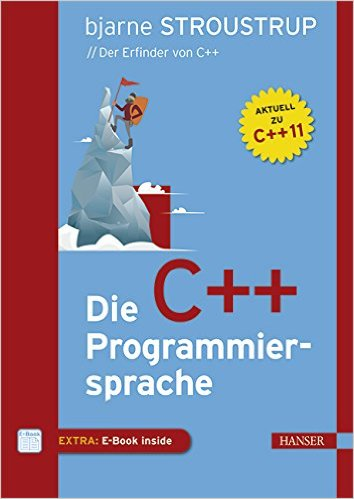
\includegraphics[width=.9\linewidth]{stroustrup.jpg}
\end{center}\end{center}
\end{column}
\begin{column}{0.5\columnwidth}
\begin{center}\begin{center}

\includegraphics[width=.9\linewidth]{schroedinger.jpg}
\end{center}\end{center}
\end{column}
\end{columns}
\end{frame}
\end{document}